\documentclass[a4paper,14pt]{article}
\usepackage{blindtext}
\usepackage[T2A]{fontenc}
\usepackage[utf8]{inputenc}
\usepackage[english,russian]{babel}
\usepackage{listings}
\usepackage{geometry}
\usepackage{amssymb}
\usepackage{amsmath}
\usepackage[14pt]{extsizes}
\geometry{left=3cm}
\geometry{right=1.5cm}
\geometry{top=2cm}
\geometry{bottom=2cm}
\pagestyle{plain}
\usepackage{pgfplots}
\usepackage{filecontents}
\usepackage{graphicx}
\usepackage{indentfirst}
\DeclareGraphicsExtensions{.png}
\graphicspath{{images/}}
\usetikzlibrary{datavisualization}
\usetikzlibrary{datavisualization.formats.functions}
\usepackage{tabularx}
\pgfplotsset{width=7 cm}
\usepackage{xcolor}
%\renewcommand{\rmdefault}{ftm}
%\usepackage{mathptmx}
\usepackage{setspace}
%\usepackage{minted}
%\полуторный интервал
\onehalfspacing
\frenchspacing

\usepackage{tocloft}
\frenchspacing
\setcounter{page}{3}
\usepackage{multirow}
\usepackage{float}
\usepackage{multirow}

\renewcommand{\cftsecdotsep}{\cftdot}
\renewcommand{\cftsecleader}{\cftdotfill{\cftsecdotsep}}
\renewcommand{\cftsubsecleader}{\cftdotfill{\cftsecdotsep}}
\renewcommand{\cftsubsubsecleader}{\cftdotfill{\cftsecdotsep}}

%\renewcommand\cftchapdotsep{\cftdot}
%\renewcommand\cftsecdotsep{\cftdot}
%\renewcommand{\cftchapleader}{\cftdotfill{\cftchapdotsep}}

% Для измененных титулов глав:
% % подключаем нужные пакеты
%\definecolor{gray75}{gray}{0.75} % определяем цвет
%\newcommand{\hsp}{\hspace{20pt}} % длина линии в 20pt
% titleformat определяет стиль
%\titleformat{\chapter}[hang]{\Huge\bfseries}{\thechapter\hsp\textcolor{black}{|}\hsp}{0pt}{\Huge\bfseries}
%\usepackage{titlesec, blindtext, color}
%\titleformat{\chapter}[hang]{\Huge\bfseries}{\thechapter\hsp\textcolor{black}{|}\hsp}{0pt}{\Huge\bfseries}

% Для листинга кода:
\lstset{ %
language=python,                 % выбор языка для подсветки
basicstyle=\small\sffamily, % размер и начертание шрифта для подсветки кода
numbers=left,               % где поставить нумерацию строк (слева\справа)
numberstyle=\tiny,           % размер шрифта для номеров строк
stepnumber=1,                   % размер шага между двумя номерами строк
numbersep=5pt,                % как далеко отстоят номера строк от подсвечиваемого кода
showspaces=false,            % показывать или нет пробелы специальными отступами
showstringspaces=false,      % показывать или нет пробелы в строках
showtabs=false,             % показывать или нет табуляцию в строках
frame=single,              % рисовать рамку вокруг кода
tabsize=4,                 % размер табуляции по умолчанию равен 2 пробелам
captionpos=t,              % позиция заголовка вверху [t] или внизу [b]
breaklines=true,           % автоматически переносить строки (да\нет)
breakatwhitespace=false, % переносить строки только если есть пробел
escapeinside={\#*}{*)},   % если нужно добавить комментарии в коде
literate={а}{{\selectfont\char224}}1
{б}{{\selectfont\char225}}1
{в}{{\selectfont\char226}}1
{г}{{\selectfont\char227}}1
{д}{{\selectfont\char228}}1
{е}{{\selectfont\char229}}1
{ё}{{\"e}}1
{ж}{{\selectfont\char230}}1
{з}{{\selectfont\char231}}1
{и}{{\selectfont\char232}}1
{й}{{\selectfont\char233}}1
{к}{{\selectfont\char234}}1
{л}{{\selectfont\char235}}1
{м}{{\selectfont\char236}}1
{н}{{\selectfont\char237}}1
{о}{{\selectfont\char238}}1
{п}{{\selectfont\char239}}1
{р}{{\selectfont\char240}}1
{с}{{\selectfont\char241}}1
{т}{{\selectfont\char242}}1
{у}{{\selectfont\char243}}1
{ф}{{\selectfont\char244}}1
{х}{{\selectfont\char245}}1
{ц}{{\selectfont\char246}}1
{ч}{{\selectfont\char247}}1
{ш}{{\selectfont\char248}}1
{щ}{{\selectfont\char249}}1
{ъ}{{\selectfont\char250}}1
{ы}{{\selectfont\char251}}1
{ь}{{\selectfont\char252}}1
{э}{{\selectfont\char253}}1
{ю}{{\selectfont\char254}}1
{я}{{\selectfont\char255}}1
{А}{{\selectfont\char192}}1
{Б}{{\selectfont\char193}}1
{В}{{\selectfont\char194}}1
{Г}{{\selectfont\char195}}1
{Д}{{\selectfont\char196}}1
{Е}{{\selectfont\char197}}1
{Ё}{{\"E}}1
{Ж}{{\selectfont\char198}}1
{З}{{\selectfont\char199}}1
{И}{{\selectfont\char200}}1
{Й}{{\selectfont\char201}}1
{К}{{\selectfont\char202}}1
{Л}{{\selectfont\char203}}1
{М}{{\selectfont\char204}}1
{Н}{{\selectfont\char205}}1
{О}{{\selectfont\char206}}1
{П}{{\selectfont\char207}}1
{Р}{{\selectfont\char208}}1
{С}{{\selectfont\char209}}1
{Т}{{\selectfont\char210}}1
{У}{{\selectfont\char211}}1
{Ф}{{\selectfont\char212}}1
{Х}{{\selectfont\char213}}1
{Ц}{{\selectfont\char214}}1
{Ч}{{\selectfont\char215}}1
{Ш}{{\selectfont\char216}}1
{Щ}{{\selectfont\char217}}1
{Ъ}{{\selectfont\char218}}1
{Ы}{{\selectfont\char219}}1
{Ь}{{\selectfont\char220}}1
{Э}{{\selectfont\char221}}1
{Ю}{{\selectfont\char222}}1
{Я}{{\selectfont\char223}}1
}

\begin{filecontents}{high_time_basic_rely_work.dat}
    1 688
    2 788
    3 917
    4 1054
    5 1284
\end{filecontents}

\begin{filecontents}{high_time_basic_rely_time.dat}
    1 25
    2 26
    3 27
    4 29
    5 31
\end{filecontents}

\begin{filecontents}{high_time_basic_data_work.dat}
    2 688
    3 732
    4 790
    5 849
\end{filecontents}

\begin{filecontents}{high_time_basic_data_time.dat}
    2 25
    3 25
    4 26
    5 26
\end{filecontents}

\begin{filecontents}{high_time_basic_cplx_work.dat}
    1 688
    2 835
    3 982
    4 1130
    5 1277
\end{filecontents}

\begin{filecontents}{high_time_basic_cplx_time.dat}
    1 25
    2 26
    3 28
    4 29
    5 31
\end{filecontents}



\begin{filecontents}{basic_rely_work.dat}
    1 507
    2 581
    3 676
    4 777
    5 947
\end{filecontents}

\begin{filecontents}{basic_rely_time.dat}
    1 27
    2 28
    3 30
    4 31
    5 34
\end{filecontents}


\begin{filecontents}{basic_data_work.dat}
    2 507
    3 539
    4 583
    5 626
\end{filecontents}

\begin{filecontents}{basic_data_time.dat}
    2 27
    3 27
    4 28
    5 29
\end{filecontents}


\begin{filecontents}{basic_cplx_work.dat}
    1 507
    2 616
    3 724
    4 833
    5 942
\end{filecontents}

\begin{filecontents}{basic_cplx_time.dat}
    1 27
    2 29
    3 31
    4 32
    5 34
\end{filecontents}






\begin{filecontents}{med_rely_work.dat}
    1 625
    2 717
    3 833
    4 959
    5 1167
\end{filecontents}

\begin{filecontents}{med_rely_time.dat}
    1 24
    2 25
    3 26
    4 28
    5 30
\end{filecontents}


\begin{filecontents}{med_data_work.dat}
    2 625
    3 665
    4 718
    5 771
\end{filecontents}

\begin{filecontents}{med_data_time.dat}
    2 24
    3 24
    4 25
    5 26
\end{filecontents}


\begin{filecontents}{med_cplx_work.dat}
    1 625
    2 759
    3 893
    4 1027
    5 1161
\end{filecontents}

\begin{filecontents}{med_cplx_time.dat}
    1 24
    2 25
    3 27
    4 28
    5 30
\end{filecontents}


\begin{filecontents}{emb_rely_work.dat}
    1 798
    2 915
    3 1064
    4 1223
    5 1489
\end{filecontents}

\begin{filecontents}{emb_rely_time.dat}
    1 21
    2 22
    3 23
    4 24
    5 26
\end{filecontents}


\begin{filecontents}{emb_data_work.dat}
    2 798
    3 849
    4 917
    5 985
\end{filecontents}

\begin{filecontents}{emb_data_time.dat}
    2 21
    3 22
    4 22
    5 23
\end{filecontents}


\begin{filecontents}{emb_cplx_work.dat}
    1 798
    2 969
    3 1140
    4 1311
    5 1482
\end{filecontents}

\begin{filecontents}{emb_cplx_time.dat}
    1 21
    2 23
    3 24
    4 25
    5 26
\end{filecontents}



\begin{document}

\begin{titlepage}

    \begin{table}
        \centering
        \footnotesize
        \begin{tabular}{cc}
            \multirow{8}{*}{
\includegraphics[scale=0.35]{bmstu.jpg}}
             &                                                                           \\
             &                                                                           \\
             & \textbf{Министерство науки и высшего образования Российской Федерации}    \\
             & \textbf{Федеральное государственное бюджетное образовательное учреждение} \\
             & \textbf{высшего образования}                                              \\
             & \textbf{<<Московский государственный технический}                         \\
             & \textbf{университет имени Н.Э. Баумана>>}                                 \\
             & \textbf{(МГТУ им. Н.Э. Баумана)}                                          \\
        \end{tabular}
    \end{table}

    \vspace{-2.5cm}

    \begin{flushleft}
        \rule[-1cm]{\textwidth}{3pt}
        \rule{\textwidth}{1pt}
    \end{flushleft}

    \begin{flushleft}
        ФАКУЛЬТЕТ Информатика и системы управления
    \end{flushleft}
    КАФЕДРА Программное обеспечение ЭВМ и информационные технологии

    \vspace{3cm}

    \begin{center}
        \textbf{Лабораторная работа № 6} \\
        \textbf{Дисциплина: <<Экономика программной инженерии>>}
        \vspace{0.5cm}
    \end{center}


    \vspace{3cm}

    \begin{flushleft}
        \begin{tabular}{ll}
            \textbf{Студент}       & Овчинникова А. П. \\
            \textbf{Группа}        & ИУ7-85Б           \\
            \textbf{Вариант}       & 15           \\
        \end{tabular}
    \end{flushleft}

    \vspace{3cm}

    \begin{center}
        Москва, 2020 г.
    \end{center}

\end{titlepage}

\setcounter{page}{2}

\subsection*{Теоретическая часть}

COnstructive COst MOdel (COCOMO – модель издержек разработки) – это алгоритмическая модель оценки стоимости разработки программного обеспечения.  Модель  COCOMO  предназначена  только  для  каскадной модели жизненного цикла.

COCOMO состоит из иерархии трех последовательно детализируемых и уточняемых форм: обычной, промежуточной и встроенной.

Трудозатраты = $C_1 \cdot EAF \cdot$(размер)$^{p_1}$

Время = $C_2 \cdot $(трудозатраты)$^{p_2}$

Для обычного режима $C_1 = 3.2, p_1 = 1.05, C_2 = 2.5, p_1 = 0.38$.
Для промежуточного режима $C_1 = 3.0, p_1 = 1.12, C_1 = 2.5, p_1 = 0.35$.
Для встроенного режима $C_1 = 2.8, p_1 = 1.2, C_1 = 2.5, p_1 = 0.32$.

$EAF = RELY \cdot DATA \cdot  CPLX \cdot ACAP \cdot AEXP \cdot PCAP \cdot VEXP \cdot LEXP \cdot TIME \cdot STOR \cdot VIRT \cdot TURN \cdot MODP \cdot TOOL \cdot SCED$

Компания  разрабатывает  программнуюсистему  управления воздушным движением. Программа обрабатывает сигналы радара и ответчика и преобразовывает их в цифровые данные, позволяющие авиадиспетчерам  назначать  курсы,  высоту  и  скорость  полетов.Разработка ведется командой высококвалифицированных специалистов в  рамках государственногоконтракта.  Предполагаемый  размер разрабатываемой системы 430000 строк кода. Система имеет высокие требования по надежности, жесткие ограничения на время выполнения и сроки разработки. Используется промежуточный режим модели.

\subsection*{Анализ  влияния различных  драйверов  затрат  на  трудоемкость  и  длительность программного проекта}

Влияние факторов RELY, DATA и CPLX на трудоемкость и время в базовом режиме модели представлено на рисунках 1 и 2 соответственно.

Влияние факторов RELY, DATA и CPLX на трудоемкость и время в промежуточном режиме модели представлено на рисунках 3 и 4 соответственно.


Влияние факторов RELY, DATA и CPLX на трудоемкость и время во встроенном режиме модели представлено на рисунках 5 и 6 соответственно.

Исходя из приведенных графиков можно сделать вывод, что наибольшее влияние на трудоемкость и время проекта оказывает драйвер затрат CPLX во всех трех режимах модели.

\newpage
\begin{figure}[!h]
    \begin{center}
      \caption{Влияние факторов RELY, DATA и CPLX на трудоемкость (базовая модель).}
      \begin{tikzpicture}
      \begin{axis}[
              xlabel = {уровни фактора},
              ylabel = {трудоемкость},
          legend pos=north west,
          ymajorgrids=true,
          width=12cm
      ]
      \addplot[color=blue, mark=square] table[x index=0, y index=1] {basic_rely_work.dat};

      \addplot[color=green, mark=square] table[x index=0, y index=1] {basic_data_work.dat};

      \addplot[color=red, mark=square] table[x index=0, y index=1] {basic_cplx_work.dat};

      \addlegendentry{RELY}
      \addlegendentry{DATA}
      \addlegendentry{CPLX}

      \end{axis}
      \end{tikzpicture}
    \end{center}
  \end{figure}



\begin{figure}[!h]
    \begin{center}
      \caption{Влияние факторов RELY, DATA и CPLX на время (базовая модель).}
      \begin{tikzpicture}
      \begin{axis}[
              xlabel = {уровни фактора},
              ylabel = {время},
          legend pos=north west,
          ymajorgrids=true,
          width=12cm
      ]
      \addplot[color=blue, mark=square] table[x index=0, y index=1] {basic_rely_time.dat};

      \addplot[color=green, mark=square] table[x index=0, y index=1] {basic_data_time.dat};

      \addplot[color=red, mark=square] table[x index=0, y index=1] {basic_cplx_time.dat};

      \addlegendentry{RELY}
      \addlegendentry{DATA}
      \addlegendentry{CPLX}

      \end{axis}
      \end{tikzpicture}
    \end{center}
  \end{figure}



  \newpage
  \begin{figure}[!h]
    \begin{center}
      \caption{Влияние факторов RELY, DATA и CPLX на трудоемкость (промежуточная модель).}
      \begin{tikzpicture}
      \begin{axis}[
              xlabel = {уровни фактора},
              ylabel = {трудоемкость},
          legend pos=north west,
          ymajorgrids=true,
          width=12cm
      ]
      \addplot[color=blue, mark=square] table[x index=0, y index=1] {med_rely_work.dat};

      \addplot[color=green, mark=square] table[x index=0, y index=1] {med_data_work.dat};

      \addplot[color=red, mark=square] table[x index=0, y index=1] {med_cplx_work.dat};

      \addlegendentry{RELY}
      \addlegendentry{DATA}
      \addlegendentry{CPLX}

      \end{axis}
      \end{tikzpicture}
    \end{center}
  \end{figure}

\begin{figure}[!h]
    \begin{center}
      \caption{Влияние факторов RELY, DATA и CPLX на время (промежуточная модель).}
      \begin{tikzpicture}
      \begin{axis}[
              xlabel = {уровни фактора},
              ylabel = {время},
          legend pos=north west,
          ymajorgrids=true,
          width=12cm
      ]
      \addplot[color=blue, mark=square] table[x index=0, y index=1] {med_rely_time.dat};

      \addplot[color=green, mark=square] table[x index=0, y index=1] {med_data_time.dat};

      \addplot[color=red, mark=square] table[x index=0, y index=1] {med_cplx_time.dat};

      \addlegendentry{RELY}
      \addlegendentry{DATA}
      \addlegendentry{CPLX}

      \end{axis}
      \end{tikzpicture}
    \end{center}
  \end{figure}




  \newpage
  \begin{figure}[!h]
    \begin{center}
      \caption{Влияние факторов RELY, DATA и CPLX на трудоемкость (встроенная модель).}
      \begin{tikzpicture}
      \begin{axis}[
              xlabel = {уровни фактора},
              ylabel = {трудоемкость},
          legend pos=north west,
          ymajorgrids=true,
          width=12cm
      ]
      \addplot[color=blue, mark=square] table[x index=0, y index=1] {emb_rely_work.dat};

      \addplot[color=green, mark=square] table[x index=0, y index=1] {emb_data_work.dat};

      \addplot[color=red, mark=square] table[x index=0, y index=1] {emb_cplx_work.dat};

      \addlegendentry{RELY}
      \addlegendentry{DATA}
      \addlegendentry{CPLX}

      \end{axis}
      \end{tikzpicture}
    \end{center}
  \end{figure}



  \begin{figure}[!h]
    \begin{center}
      \caption{Влияние факторов RELY, DATA и CPLX на время (встроенная модель).}
      \begin{tikzpicture}
      \begin{axis}[
              xlabel = {уровни фактора},
              ylabel = {время},
          legend pos=north west,
          ymajorgrids=true,
          width=12cm
      ]
      \addplot[color=blue, mark=square] table[x index=0, y index=1] {emb_rely_time.dat};

      \addplot[color=green, mark=square] table[x index=0, y index=1] {emb_data_time.dat};

      \addplot[color=red, mark=square] table[x index=0, y index=1] {emb_cplx_time.dat};

      \addlegendentry{RELY}
      \addlegendentry{DATA}
      \addlegendentry{CPLX}

      \end{axis}
      \end{tikzpicture}
    \end{center}
  \end{figure}


\newpage
Исследуем влияние драйверов затрат на трудоемкость и сроки разработки при наличии более жестких ограничений на время выполнения (высокий уровень фактора TIME). Будем использовать базовую модель (рисунки 7 и 8). Из приведенных графиков видно, что при наличии более жестких ограничений на время выполнения драйвер затрат CPLX также оказывает наибольшее влияние и на время реализации, и на трудоемкость.



\begin{figure}[!h]
  \begin{center}
    \caption{Влияние факторов RELY, DATA и CPLX на трудоемкость (встроенная модель).}
    \begin{tikzpicture}
    \begin{axis}[
            xlabel = {уровни фактора},
            ylabel = {трудоемкость},
        legend pos=north west,
        ymajorgrids=true,
        width=12cm
    ]
    \addplot[color=blue, mark=square] table[x index=0, y index=1] {high_time_basic_rely_work.dat};

    \addplot[color=green, mark=square] table[x index=0, y index=1] {high_time_basic_data_work.dat};

    \addplot[color=red, mark=square] table[x index=0, y index=1] {high_time_basic_cplx_work.dat};

    \addlegendentry{RELY}
    \addlegendentry{DATA}
    \addlegendentry{CPLX}

    \end{axis}
    \end{tikzpicture}
  \end{center}
\end{figure}


\begin{figure}[!h]
    \begin{center}
      \caption{Влияние факторов RELY, DATA и CPLX на время при наличии более жестких ограничений на время выполнения(встроенная модель).}
      \begin{tikzpicture}
      \begin{axis}[
              xlabel = {уровни фактора},
              ylabel = {время},
          legend pos=north west,
          ymajorgrids=true,
          width=12cm
      ]

      \addplot[color=blue, mark=square] table[x index=0, y index=1] {high_time_basic_rely_time.dat};

      \addplot[color=green, mark=square] table[x index=0, y index=1] {high_time_basic_data_time.dat};

      \addplot[color=red, mark=square] table[x index=0, y index=1] {high_time_basic_cplx_time.dat};

      \addlegendentry{RELY}
      \addlegendentry{DATA}
      \addlegendentry{CPLX}

      \end{axis}
      \end{tikzpicture}
    \end{center}
  \end{figure}

\newpage
\subsection*{Анализ проекта по управлению воздушным движением}

Настройки параметров проекта представлены на рисунке \ref{fig:settings}. В качестве языка программирования выберем С++. Декомпозиция работ по созданию ПО представлена на рисунке \ref{fig:decompos}. Распределение работ и времени по стадиям жизненного цикла представлено на рисунке \ref{fig:cycle}. Диаграмма привлечения сотрудников представлена на рисунке \ref{fig:workers}. 

При оценке стоимости человеко-месяца равной 60000 рублей, бюджет проекта был предварительно оценен в 4 440 000 рублей.


\begin{figure}[!h]
   \center{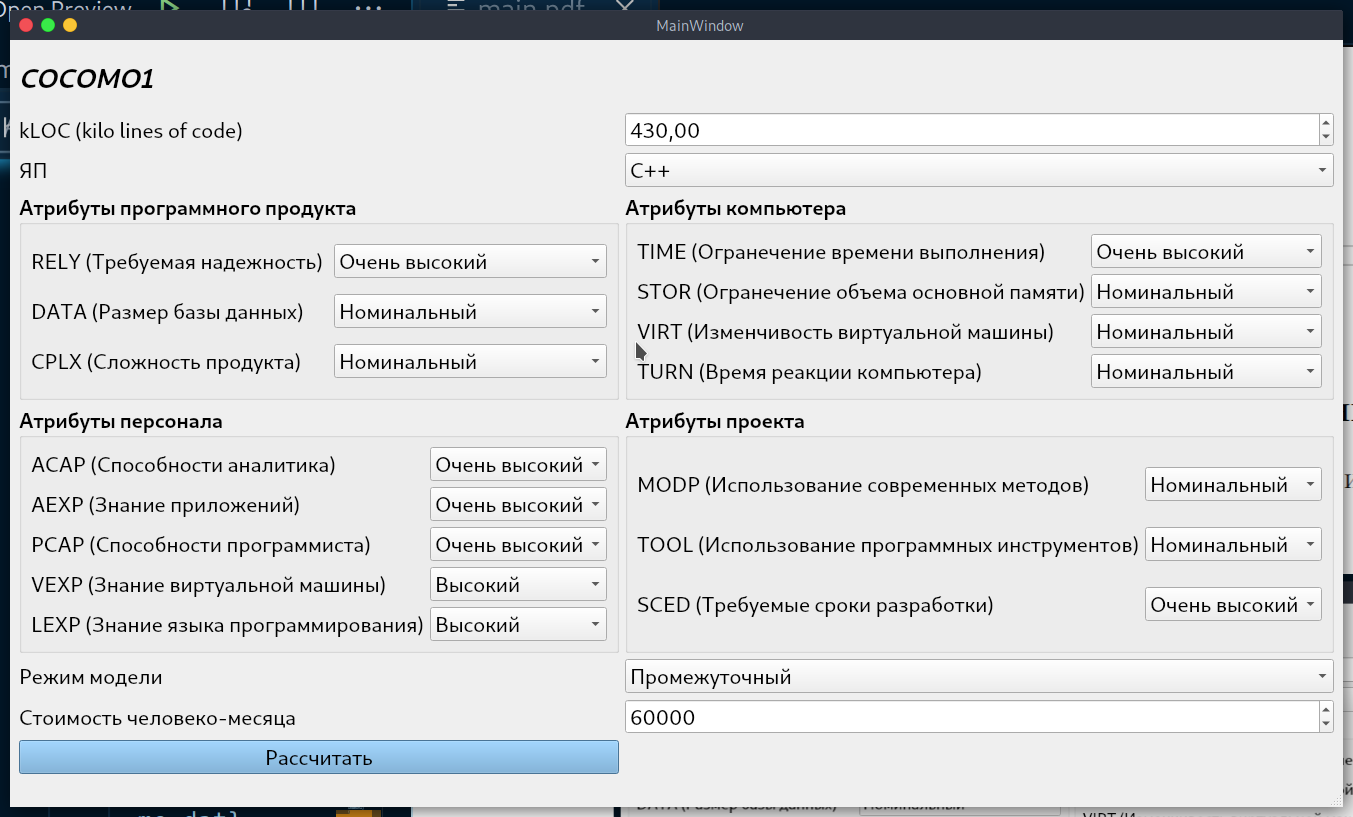
\includegraphics[width=16cm]{settings}}
    \caption{Настройки параметров проекта.}
    \label{fig:settings}
\end{figure}

\newpage
\begin{figure}[!h]
    \center{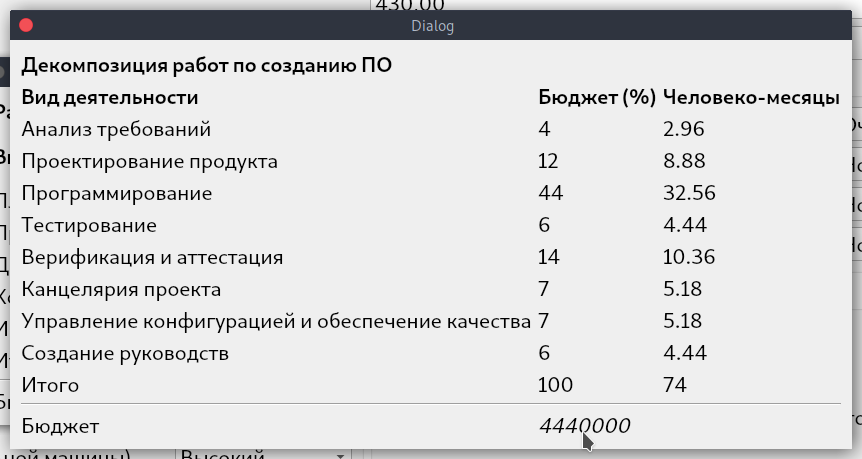
\includegraphics[width=16cm]{decompos}}
     \caption{Декомпозиция работ по созданию ПО.}
     \label{fig:decompos}
 \end{figure}

 \begin{figure}[!h]
    \center{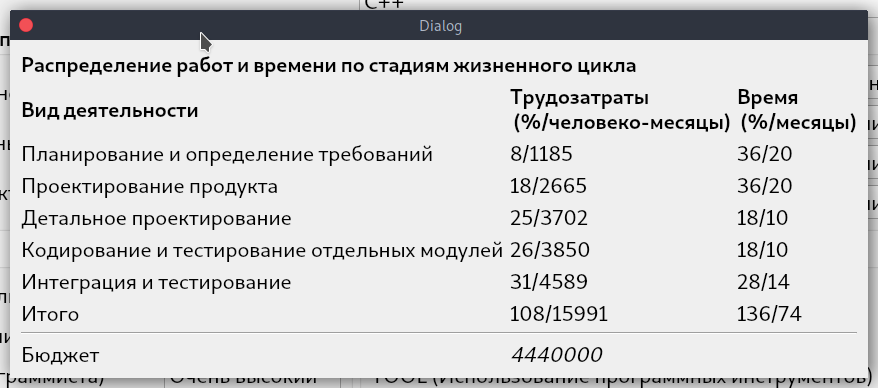
\includegraphics[width=16cm]{cycle}}
     \caption{Декомпозиция работ по созданию ПО.}
     \label{fig:cycle}
 \end{figure}

 \begin{figure}[!h]
    \center{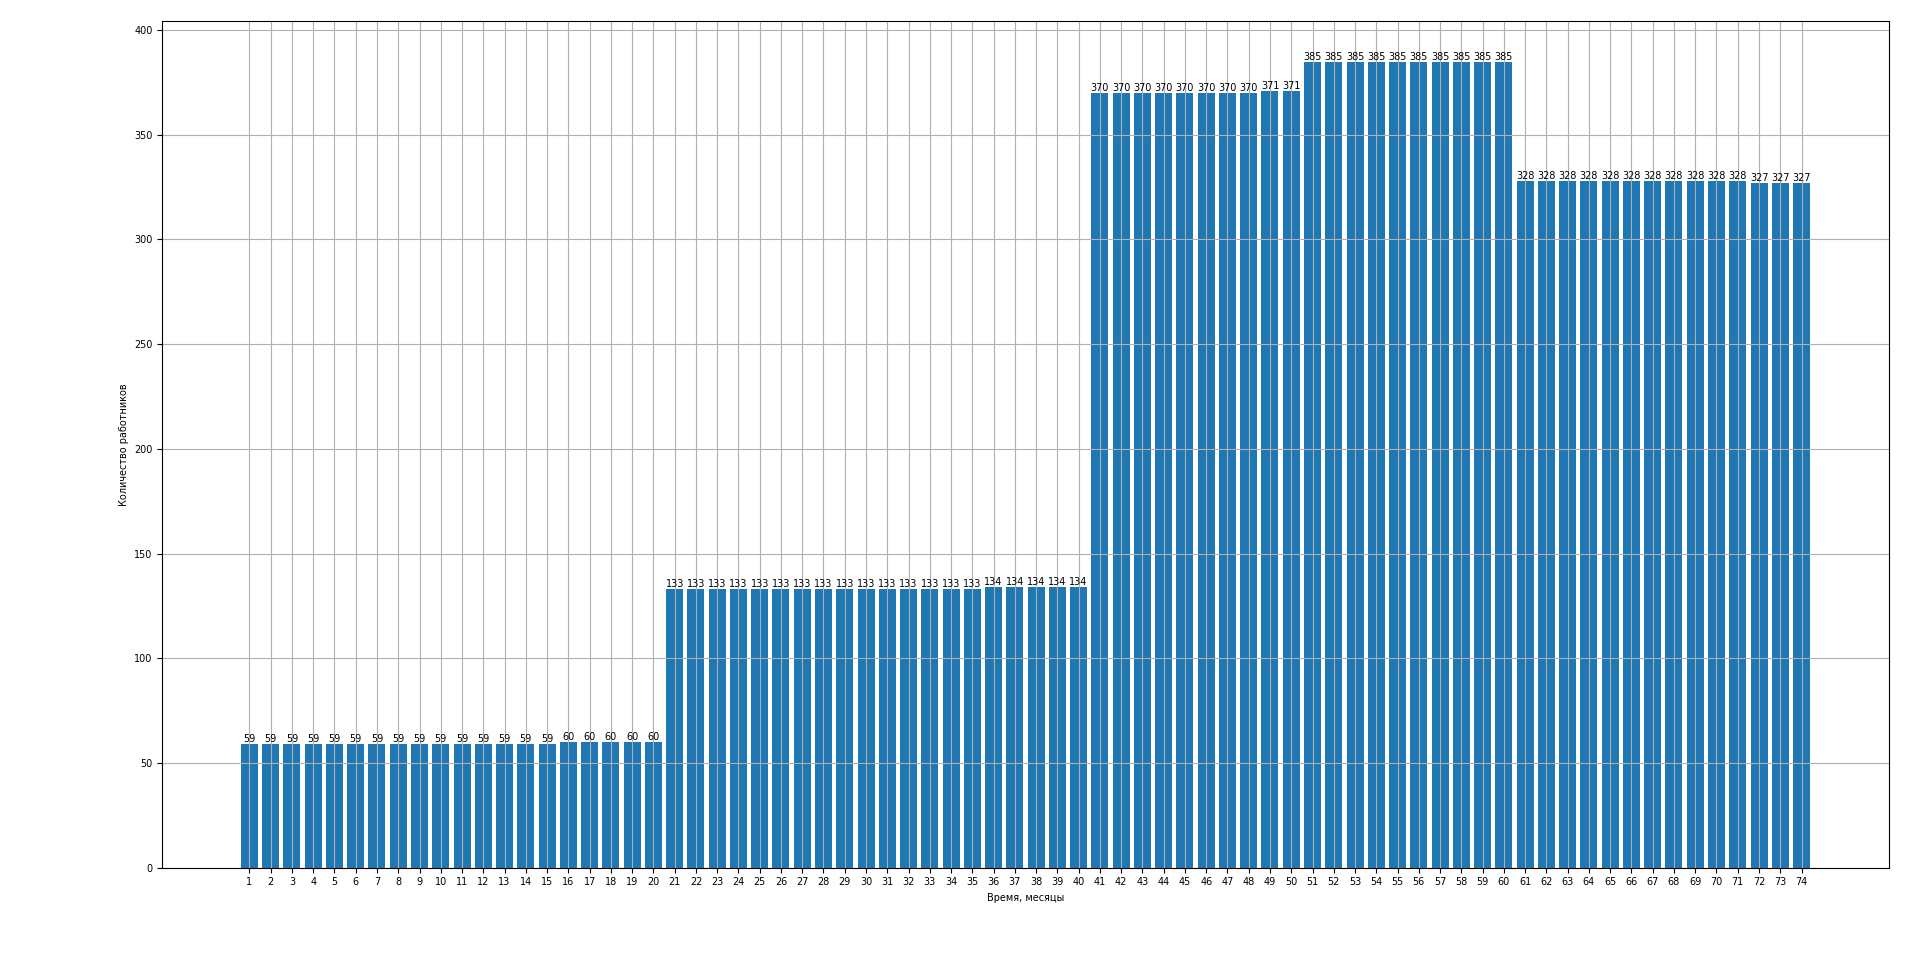
\includegraphics[width=16cm]{workers}}
     \caption{Численность команды проекта.}
     \label{fig:workers}
 \end{figure}

\newpage
\subsection*{Заключение о применимости модели COCOMO для решения поставленной задач}

Использование методики COCOMO позволяет дать первичную оценку проекта, используя только информацию о количестве строк кода (KLOC).
Методика COCOMO промежуточного и встроенного уровня требует значительных усилий на проведение предварительной оценки, а результаты оценки базового метода недостаточно точны. Поэтому применима только для средних и крупных проектов.

Кроме того, для коммерческих проектов метод COCOMO приводит к завышенным значениям оценок. Поэтому метод COCOMO применяется только к разработке технического программного обеспечения.

Однако стоит учитывать, что в настоящее время существует методика COCOMO2, которая способна учитывать особенности конкретного ПО, такие как его интерфейс, данные и их движение внутри програмнного комплекса, а поэтому может дать более точную оценку трудозатрат и времени разработки проекта.

\end{document}
